\chapter{Physics Objects}
\label{chap:objects}

In this chapter the algorithms used to reconstruct analysis objects and
quantities from individual measurements from different parts of the CMS detector
are described.

\begin{figure}[htbp]
  \centering
  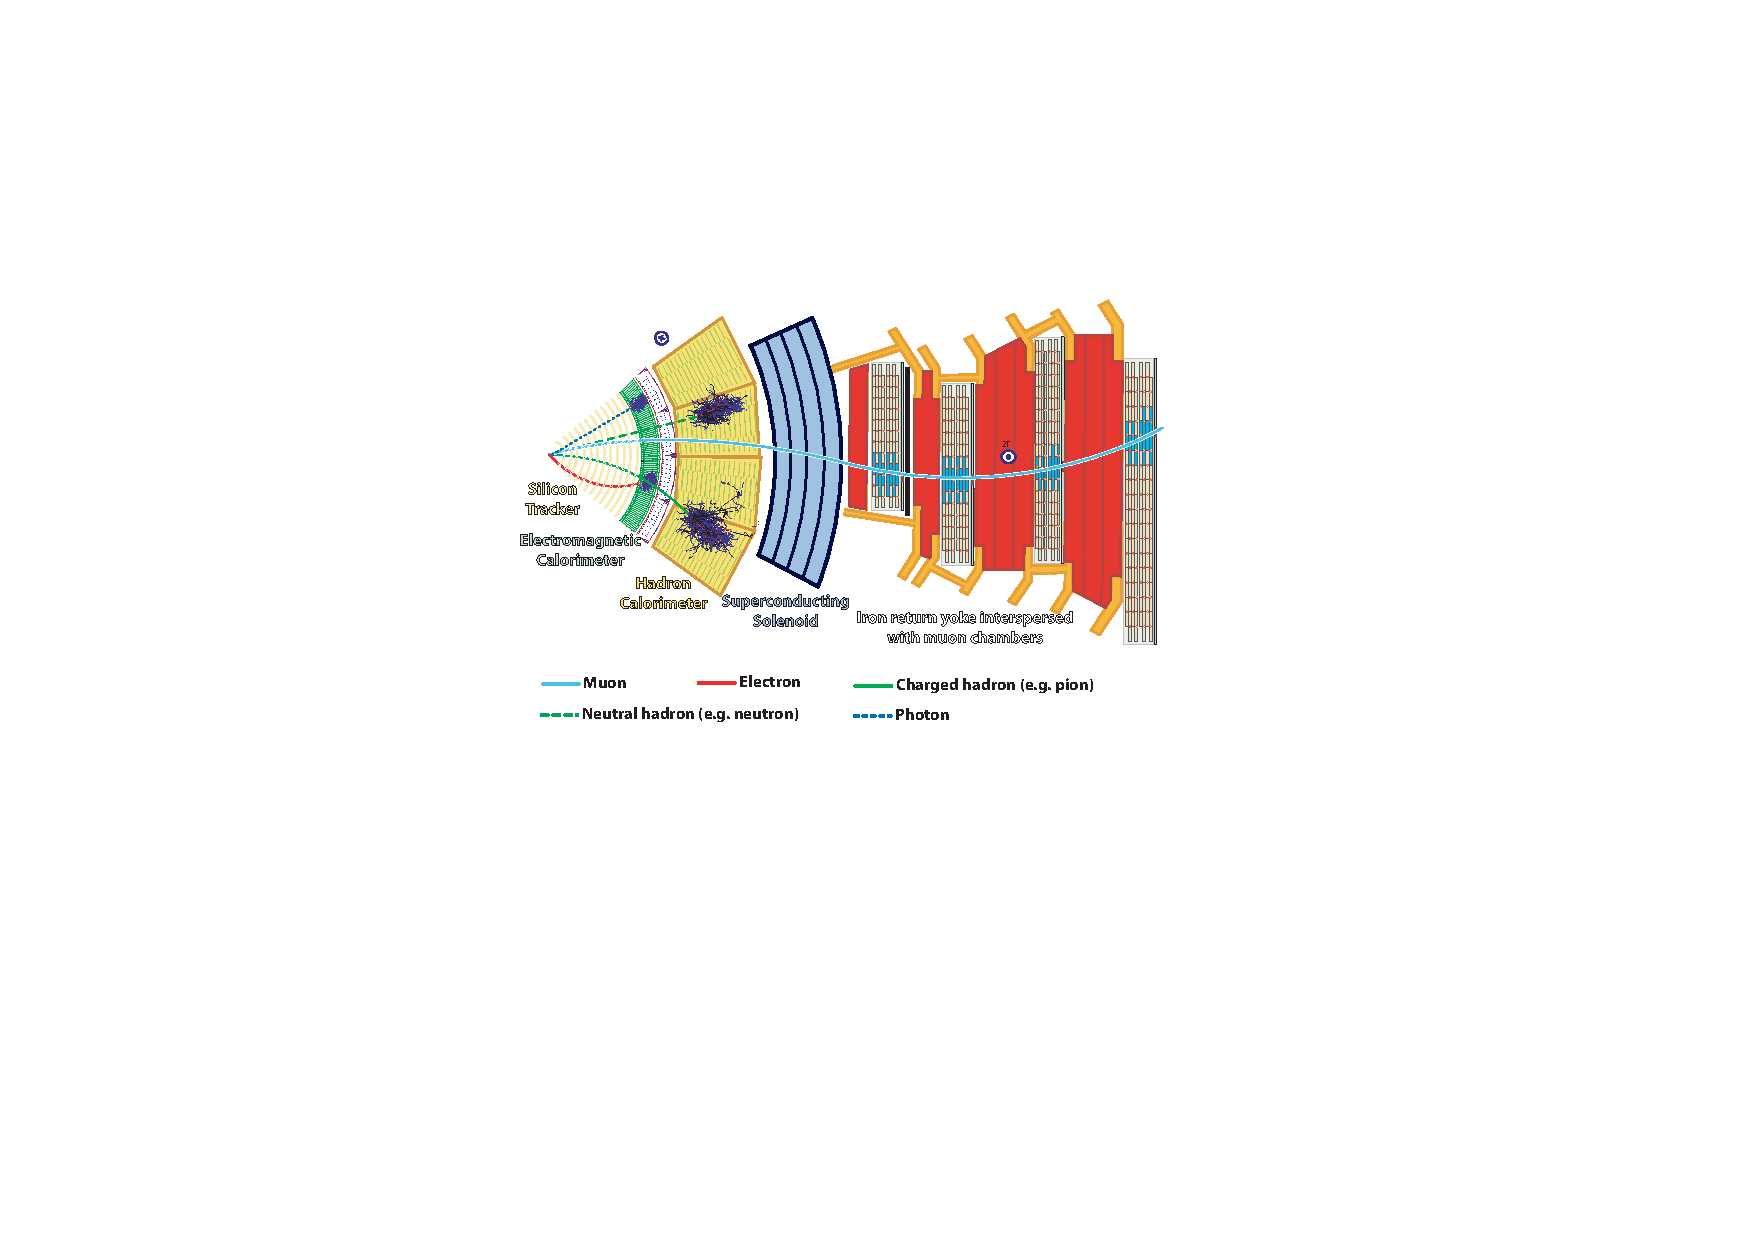
\includegraphics[trim=8cm 8cm 9cm 5cm, width=\textwidth]{slice}
  \caption{The path of different particles through a cross section of the CMS
detector. From \cite{cmsSlice}.}
  \label{reco:crosssec}
\end{figure}

\FigureRef{reco:crosssec} shows a cross section of \ac{CMS} superimposed with the
typical paths of several different particles and their interactions with the
subdetectors of \ac{CMS}.  This chapter describes how the information
from each subdetector is combined to identify and reconstruct the particles.

\section{Electrons}

Electrons are important physics objects in CMS as they provide easy-to-identify
signatures and their energy can be measured with a good resolution. This section
will describe the electron reconstruction algorithms used to produce electron
candidates, and the identification variables used to discriminate between real
electron candidates and their backgrounds.

\subsection{Reconstruction}
Electrons are reconstructed in CMS using information from the pixel detector,
silicon strip tracker and the ECAL.
The first step of the reconstruction is to collect together energy deposits in
the ECAL. Next, the path of the electron though the tracker is reconstructed and
matched to the energy deposits in the ECAL.

\subsubsection{Electron Clustering}

In addition to ionisation energy losses and multiple Colomb scattering,
electrons will suffer large energy losses while traversing the inner detector
by a process called bremsstrahlung. 
As electrons collide with the atomic nuclei, the nuclear electric field
declerates the electron, and the energy change appears in the form of an photon
\cite{perkins}.  
The photon may then undergo pair production, in the field of a nucleus to
conserve momentum, to produce a electron-positron pair.
As the electron traverses the CMS tracker, the strong magnetic
field causes the path to be curved in the azimuthal, $\phi$,
direction, so that when the electron reaches the \acs{ECAL} it is accompanied
by a ``spray'' of electromagnetic energy spread over a narrow strip in the phi direction.
\FigureRef{fig:brem} shows the fraction of energy radiated by bremsstrahlung for
electrons of energy $10$, $30$ and \unit{$50$}{\GeV} \cite{eReco}.

\begin{figure}[htbp]
  \centering
  \includegraphics[width=0.7\textwidth]{brem}
  \caption{Average fraction of electron energy, $E^{e}$, radiated away as bremsstrahlung
photons, $\sum E_{brem}^{\gamma}$ for electrons of energy 10, 30 and
\unit{50}{\GeV}. From \cite{eReco}.}
\label{fig:brem}
\end{figure}

To measure the electron energy, the separated deposits of energy need to be
collected together, using ``super-clustering'' algorithms. 

In the barrel a ``hybrid'' algorithm is used. The hybrid algorithm proceeds by
identifying crystals with energies above a certain threshold, that will act as
seeds. The algorithm then forms $1\times3$ or $1\times5$ crystal ``dominos'' in
the $\eta\times\phi$ respectivly, centred on the seed crystal, depending on the
energy within the domino. The dominos are then collected together in the $\phi$
direction, up to an extension of \unit{0.3}{\rad}, to form clusters of dominos.
This is demonstrated in \FigureRef{fig:hybrid} \cite{eECAL}.

\begin{figure}[htbp]
  \centering
  \includegraphics[width=0.95\textwidth]{hybridalgo}
  \caption{Demonstration of the clustering of dominos in the hybrid algorithm.
From \cite{eECAL}.  The algorithm starts on the seed crystal and clusters
$1\times3$ and $1\times5$ dominos to form the first subcluster. The algorithm continues to search
by stepping in phi and identifies a second subcluster.}
  \label{fig:hybrid}
\end{figure}

A ``multi5x5'' algorithm is used in the ECAL endcaps. Energy is collected in
$5\times5$ crystal arrays which are then collected together, if their position lies on
a narrow $\phi$ road, to form superclusters.

\subsubsection{Electron Seeding}
The superclusters are then used to select seeds for the track reconstruction.
Starting with a supercluster that passes a \pt threshold and a hadronic veto,
the trajectory of the electron is propagated back through the magnetic field and
matched to pairs or triplets of hits in the inner tracker that act as trajectory
seeds.  If the trajectory seeds fall within a window of the super cluster path
under either charge hypothesis, they are selected and used to seed the track
reconstruction.  This ECAL-driven seeding is complemented by a tracker-driven
seeding algorithm.  This starts with high purity tracks and extrapolating them
outwards to the ECAL and is more effective for lower \pt electrons.

Seeds from both of the algorithms are collected and merged into a single
collection, which is then used to seed the electron track reconstruction.

\subsubsection{Electron Track Reconstruction}
The track reconstruction is based on a combinatorial Kalman filter \cite{kalman},
with the electron energy losses described using Bethe-Heitler
modelling \cite{bethe}.
The track reconstruction starts from a trajectory seed, from which a tree of
possible track candidates is built. 

The Kalman filter is a two step process. In the propagation step, track
candidates are extrapolated to the next layer of the detector, while taking into
 account energy losses due to bremsstrahlung and Coulomb scattering.  In
the update step, the extrapolated track candidate is combined with the observed
trach hit in that layer and the track parameters are updated. 

The collected hits are passed to the \ac{GSF} for a final fitting and estimation
of the track parameters \cite{cmsgsf}. The \ac{GSF} algorithm is similar to the
Kalman filter but energy losses are now described by a weighted sum of Gaussian
distributions \cite{gsf}.
% corrections

\subsection{Backgrounds to Prompt Electrons}
In addition to prompt electrons, the electron candidates from the reconstruction
algorithms will contain background signatures, either fake electrons or unwanted
real electrons produced via some background process.

There are two main processes that may produce signatures in the detector that
may be mistakenly identified as an electron and an additional
two processes that may produce real electrons \cite{nikos}.

\subsubsection{Charged hadrons that shower early in the ECAL}
A charged pion will leave a track, that will appear similar to an non-radiating
electron track.
If the pion were to produce a hadronic shower early in the ECAL
the energy deposits in the ECAL could be wrongly identified as an
electromagnetic shower.
As an example, the charge exchange process,
\begin{align}
\Ppiminus + \Pproton \to &\Ppizero + \Pneutron \nonumber \\
                         &\to \Pphoton\Pphoton
\end{align}
would be almost indistiguishable from an electron shower.
The electron reconstruction algorithm would combine the
track and electromagnetic shower to form an electron candidate.

\subsubsection{\HepProcess{\Ppipm \Ppizero} overlap}
A charged pion within a jet will produce a charged track whereas a neutral pion
will quickly decay to a pair of photons. If the electromagnetic clusters from
the \Ppizero are matched to the track from the charged hadron, the electron
reconstruction algorithm may form an electron candidate.

\subsubsection{Electrons from hadronic decays}
Heavy flavour quarks may decay semi-leptonically to produce real electrons. These
electrons will tend to be less well isolated than prompt electrons from \PW
decays.

\subsubsection{Electrons from conversions}
As stated previously, a neutral pion will produce a pair of photons. As the
photons traverse the tracker material they may convert to produce a pair of real
electrons. 
\FigureRef{fig:conversion} shows an example of a prompt electron and a pair of
electrons from photon conversion.  Electrons from photon conversions will appear
to have a large distance of closest approace to the beam spot, $d_0$.
The electrons will also tend to have missing hits in the inner tracker close to
the interaction point.
There may also be a partner track nearby with an opposite charge.
\begin{figure}[htbp]
  \centering
  \begin{subfigure}{0.49\textwidth}
    \centering
    \includegraphics[trim = 35mm 40mm 30mm 30mm, clip,width=\textwidth]{doca_electron}
    \caption{Prompt electron.}
    \label{fig:electron_path}
  \end{subfigure}
  \begin{subfigure}{0.49\textwidth}
    \centering
    \includegraphics[trim = 35mm 40mm 30mm 30mm, clip,width=\textwidth]{doca}
    \caption{Converted photon.}
    \label{fig:photon_path}
  \end{subfigure}
  \caption{Tracks from an electron and a coverted photon in the inner tracker. Modified from \cite{eConver}.}
  \label{fig:conversion}
\end{figure}


\subsection{Electron Identification}
Electron identification is based on a limited number of variables.

\subsubsection{Shape variable}

$\sigma_{\eta\eta}$ is the width of the electron shower in the $\eta$
direction,
\begin{equation}
\sigma_{\eta\eta} = 
\sum_{\text{crystals}} \left(\eta_{i} - \eta{s}\right)^{2}
\frac{E_{i}}{E_{\text{seed cluster}}}.
\end{equation}
This variable discriminates between electrons and jets, as a hadronic
shower from a jet or a pair of photons from a \Ppizero will tend to produce a
wider electromagnetic shower in the $\phi$ direction than a prompt electron.

\subsubsection{Hadronic energy}
The variable $\frac{H}{E}$ is the ratio of the energy deposited in the HCAL
tower behind the electromagnetic seed cluster to the energy of that seed
cluster. This variable offers some discrimination against early showering
hadrons as some of the energy will tend to leak into the HCAL.

\subsubsection{Angular separation of track and supercluster}
$\Delta\phi$ and $\Delta\eta$ represent the angular separation between the
trajectory of the reconstructed \ac{GSF} track, extrapolated to the ECAL, and
the ECAL supercluster in the $\phi$ and $\eta$ direction respectively.

\begin{align}
|\Delta\eta| &\equiv |\eta_{\text{SC}} - \eta_{track}|\\
|\Delta\phi| &\equiv |\phi_{\text{SC}} - \phi_{track}|
\end{align}

These variables are discriminating against accidental matching to the track and
super cluster.

\subsubsection{Isolation quantities}
For the calorimeter quantities the isolation is defined as the sum of energy in
a cone of $\Delta R = 0.3 $\todo{define this somewhere} centred on the super
cluster, where the energy deposits associated with the electron have been
removed, divided by the candidate electron \Pt.

The track isolation is defined as the sum of the \Pt of Kalman filter tracks in
a cone of $\Delta R = 0.3 $ centred on the candidate electron, divided by the
candidate electron \Pt.

Isolation offers very good discrimination between electrons and hadrons, as
hadrons that are mistakenly identified as an electron will tend to be
accompanied by other particles, whereas prompt electrons will usually be well
isolated.

\subsubsection{Conversion rejection}
Three further variables are included to reject electrons that are produced from
photon conversions. They are the number of missing hits, $\Delta\cot\theta$ and
$dist$. 

The number of missing hits is simply the number of layers in the inner
tracker where an expected hit from the track reconstruction is not detected by
the detector.

Two other variables are based on conversion partner tracks.
Conversion partner tracks are track candidates that are within a cone of $\Delta
R < 0.3$ around the electron candidate track, and have an opposite charge. 
$\Delta\cot\theta$ is defined as,
\begin{equation}
\Delta \cot \theta \equiv \cot(\theta_{\text{KF}}) - \cot(\theta_{\text{\ac{GSF}}}),
\end{equation}
where $\theta_{KF}$ and $\theta_{\ac{GSF}}$ are the polar angle of the conversion
partner track and the \ac{GSF} track of the electron respectively.
The $dist$ variable is the distance between the two tracks at the point where
they are parallel to one another in the $x-y$ plane as shown in \FigureRef{fig:dist}.

\begin{figure}[htbp]
  \centering
  \begin{subfigure}{0.45\textwidth}
    \centering
    \includegraphics[trim = 40mm 40mm 40mm 40mm, clip,width=\textwidth]{dist_m}
    \caption{$dist<0$.}
    \label{fig:dist_m}
  \end{subfigure}
  \begin{subfigure}{0.45\textwidth}
    \centering
    \includegraphics[trim = 40mm 40mm 40mm 40mm, clip,width=\textwidth]{dist_p}
    \caption{$dist>0$.}
    \label{fig:dist_p}
  \end{subfigure}
  \caption{$dist$ is the distance between the the two tracks where they are
parallel. $dist$ is defined to be negative in the case that the tracks overlap
and positive otherwise. Modified from \cite{eConver}.} 
\label{fig:dist}
\end{figure}



\subsubsection{Electron identification working points}

Several sets of cuts have been produced for CMS analyses with different
efficiencies in mind. The cut values are summarised in \TableRef{tab:electronwp}
\cite{nikos}.

The cuts can be split in to three categories, ID Cuts, isolation cuts and
conversion rejection cuts. Different sets of cut values are used for electrons in the
ECAL barrel and endcap. The cut values are obtained by simultaneous optimisation
for electron \unit{\ET=25}{\GeV}. Although the efficiency and and the background
rejection of the cuts is dependent on the \ET of the electron, the cut values
obtained are found to be effective in the range \unit{15-100}{\GeV}.\cite{nikos}

\begin{table}[htbp]
  \begin{center}
    \begin{tabular}{lllllll} 
\toprule
Efficiencies& $95\%$& $90\%$& $85\%$& $80\%$& $70\%$& $60\%$\\
\midrule
\multicolumn{7}{l}{\emph{Conversion Rejection Cuts}}\\ 
Missing Hits $\leq$& 1& 1& 1& 0& 0& 0\\
Dist& N/A& 0.02& 0.02& 0.02& 0.02& 0.02\\
$\Delta\cot\theta$& N/A& 0.02& 0.02& 0.02& 0.02& 0.02\\
\midrule
\multicolumn{7}{l}{Barrel}\\ 
\multicolumn{7}{l}{\emph{Relative Isolation Cuts}} \\
trackRel03& 0.15& 0.12& 0.09& 0.09& 0.05& 0.04\\
ecalRel03& 2.00& 0.09& 0.08& 0.07& 0.06& 0.04\\
hcalRel03& 0.12& 0.10& 0.10& 0.10& 0.03& 0.03\\
\multicolumn{7}{l}{\emph{Electron ID Cuts}} \\
$\sigma_{i\eta i\eta}$& 0.01& 0.01& 0.01& 0.01& 0.01& 0.01\\
$\Delta \phi$& - & - & 0.06& 0.06& 0.03& 0.025\\
$\Delta \eta$& 0.007& 0.007& 0.006& 0.004& 0.004& 0.004\\
HoE& 0.15& 0.12& 0.04& 0.04& 0.025& 0.025\\
\midrule
\multicolumn{7}{l}{End Cap}\\ 
\multicolumn{7}{l}{\emph{Relative Isolation Cuts}} \\
trackRel03& 0.08& 0.05& 0.05& 0.04& 0.025& 0.025\\
ecalRel03& 0.06& 0.06& 0.05& 0.05& 0.025& 0.02\\
hcalRel03& 0.05& 0.03& 0.025& 0.025& 0.02& 0.02\\
\multicolumn{7}{l}{\emph{Electron ID Cuts}} \\
$\sigma_{i\eta i\eta}$& 0.03& 0.03& 0.03& 0.03& 0.03& 0.03\\
$\Delta \phi$& - & - & 0.04& 0.03& 0.02& 0.02\\
$\Delta \eta$& 0.01& 0.009& 0.007& 0.007& 0.005& 0.005\\
HoE& 0.07& 0.05& 0.025& 0.025& 0.025& 0.025\\
\bottomrule
    \end{tabular}
    \caption{Electron selection variables and
corresponding cut values for several different efficieny working points
\cite{nikos}.}
  \end{center}
\label{tab:electronwp} 
\end{table}

\subsection{Charge Identification}
\label{sec:charge}
The charge of an electron can be identified by studying how the electron
trajectory is bent in the magnetic field as the electron passes through the
silicon tracker. This can be made difficult by conversion of bremsstrahlung
photons when they are radiated early.

Within CMS, three methods of charge identification have been developed based on
the \ac{GSF} track charge, the general track charge and the supercluster charge. The
\ac{GSF} track charge is simply the sign of the curvature of the \ac{GSF} fit of the
electron track. The general track charge is found by matching the \ac{GSF} track with
a general Kalman filter track by asking for shared hits in the pixel tracker. 
The supercluster charge is obtained by finding the sign of the $\phi$ difference
between the supercluster position and the first hit of the electron track.

At the \PZ peak, a charge mis-identification rate of \unit{3}{\%} \cite{eReco}
is measured when using the electron trajectory from the \ac{GSF} fit.  A sample with
improved charge identification can be obtained by using a majority method, that
combines the three measurements and assigns the sign from the 2 estimates out of
three that are in agreement, or by requiring that all three methods for
assigning charge are in agreement and discarding the event otherwise.

\section{Muons and Taus}
Muons and taus are not used in much detail throughout the analyses presented in
this thesis. Their reconstruction will only be briefly described. 
Muons are reconstructed from information in the muon chambers and the silicon
tracker.  Full details of the muon reconstruction are described in \cite{}.
Taus may decay leptonically or hadronically. Leptonically decaying taus will
decay to muons or electrons and may be indistinguishable from those prompt
leptons. The reconstruction algorithms for taus are described in \cite{}.

\section{Missing Energy} 
Neutrinos are weakly interacting neutral particles that escape the
detector without being directly detected by any of the detector components. 
Instead they can be indirectly detected by measuring the total momentum of the
reconstructed particles in an event.
An imbalance in the total momentum of the event can be assigned to undetected
particles. This is called the missing energy in the event.

Unfortunately, the initial longitudinal momentum of the event is not known in a
hadron collider. So, instead the imbalance in only the transverse plane is
considered. This is the missing transverse energy, \ETm, and is defined as
the negative vector sum of all final state particles in an event,
\begin{equation}
\vec{E}_^{\text{miss}}{\text{T}} = -\sum_i^{\text{particles}} \vec{p}_{T}^{i}.
\end{equation}

There are several ways of measuring the missing transverse energy.
Calo \ETm is measured by creating pseudo-particles from the energies and
direction of deposits in the calorimeter towers. The muons are included by
adding their \Pt to the calculation and removing their energy deposit in the
calorimeter. The calo \ETm is then the sum of the transverse energy of the
pseudo particles.
Track \ETm extends calo \ETm to include the track \Pt and remove the energy
deposit for each track in the event.
Particle Flow \ETm (PF \ETm) is the sum of the transverse energies of all the
reconstructed particle flow particles.\cite{PF}

\subsection{Particle Flow at CMS}

The particle-flow event reconstruction attempts to reconstruct and identify all
stable particles in an event by combining information from all CMS
sub-detectors. The particle reconstruction and identification starts with
collecting information from each sub-detector to form elements such as tracks
and energy clusters in the calorimeters. These basic 'elements' are then
combined to form blocks which are then interpreted in terms of particles by the
particle flow algorithm. A list of individual particles is then returned from
the algorithm which can be used to study the event in greater detail by,
amongst other things, building jets, tagging b quarks and calculating missing
transverse energy.\cite{PF}

The first step of the particle-flow reconstruction algorithm is to collect the
fundamental elements. The elements consist of charged particle tracks from the
tracker, clusters of energy deposition in the calorimeters and muon tracks.

As a particle traverses the detector it may interact with many CMS sub-detectors
creating several particle-flow elements. A link algorithm is used to connect
the elements together to form blocks that typically contain 1, 2 or 3 elements.
The algorithm returns a distance between the elements as a measure of the
quality of the link. The final step of the particle flow algorithm is to
reconstruct and identify particles from each block of linked elements.\cite{PF}

Once the event has been fully reconstructed with the particle flow technique
the missing transverse energy (\ETm) in the event can be easily computed by
summing up the transverse momentum of all the reconstructed particles.\cite{PF}

\section{Jets}
Jets are reconstructed from information in the tracker and the calorimeters.
Jets are clustered using an anti-$k_T$ algorithm  with a size of
$R=0.5$.

There are four collections of jets produced by the event reconstruction
algorithms at CMS, Calorimeter (Calo) jets, Particle Flow (PF) Jets, Jet Plus
Tracks (JPT) jets and track jets. Calo jets are jets reconstructed from energy
deposits in the ECAL and HCAL. JPT jets extend the Calo jets to include
information from the tracker to give an enhanced \pT resolution. PF jets are
produced by the particle flow algorithm\cite{PF}. Track jets are reconstructed from
tracks in the silicon tracker.

